\documentclass{standalone}
\usepackage[dvipsnames]{xcolor}
\usepackage{amsmath}
\usepackage{tikz}
\usetikzlibrary{chains}
\usetikzlibrary{shapes}
\usetikzlibrary{arrows}
\usetikzlibrary{decorations.pathreplacing,shapes}

\newcommand\kk[1]{\textcolor{RoyalBlue}{\text{\textup{\textbf{\texttt{#1}}}}}}
\newcommand\cc[1]{\textcolor{Sepia}{\text{\textup{\textbf{\texttt{#1}}}}}}

\begin{document}

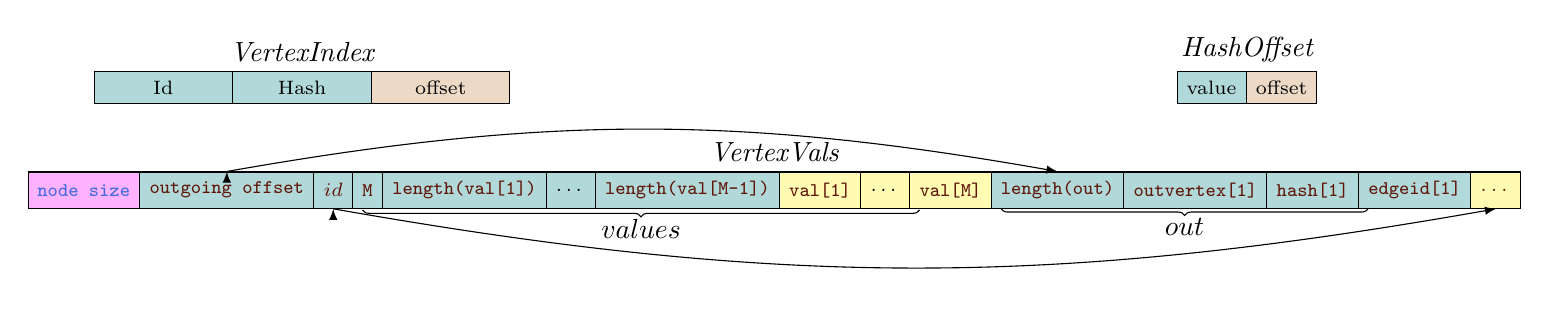
\begin{tikzpicture}[>=latex,auto]
\begin{scope}[node distance=0pt]
\def\width{9ex}

\tikzstyle{frame}=[
	font=\scriptsize,
	%text width=7ex,
	draw,
	rectangle split,
	rectangle split parts=20,
	rectangle split part align={center, left},
	rectangle split empty part height=0ex,
	rectangle split empty part depth=0ex,
	rectangle split empty part width=0ex,
	start chain=going right,
	rectangle split horizontal
]

%%MAIN
\node (main) [frame,
	rectangle split parts=15,
	rectangle split part fill={Fuchsia!30,
							   teal!30,
							   teal!30,
							   teal!30,teal!30,teal!30,teal!30,
							yellow!30,yellow!30,yellow!30,
							teal!30,
							teal!30,teal!30,teal!30,yellow!30}
] at (0,.7) {%
\nodepart{one} 
    \centering \kk{node size}
\nodepart{two} \centering \cc{outgoing offset}
\nodepart{three} \centering \cc{$id$}
    \nodepart{four} \cc{M}
    \nodepart{five} \cc{length(val[1])}
    \nodepart{six} \dots
    \nodepart{seven}\cc{length(val[M-1])}
    \nodepart{eight}\cc{val[1]}
    \nodepart{nine} \dots
    \nodepart{ten}\cc{val[M]}
		\nodepart{eleven}\cc{length(out)}
   		\nodepart{twelve} \cc{outvertex[1]}
   		\nodepart{thirteen} \cc{hash[1]}
   		\nodepart{fourteen} \cc{edgeid[1]}
   		\nodepart{fifteen}\cc{$\dots$}
};

%% SORT
\node (sort) [frame,
	rectangle split parts=3,
	text width=10ex,
	align=center,
	rectangle split part fill={teal!30,teal!30,brown!30}
] at (-6,2) {
\nodepart{one} Id
\nodepart{two} Hash
\nodepart{three} offset
};

\node (qsort1) [frame,
	rectangle split parts=2,
	rectangle split part fill={teal!30,brown!30} 
] at (6,2) {%
\nodepart{one} \centering value
\nodepart{two} offset
};


\node[above=0 pt of main.north,anchor=south,font=\itshape] {VertexVals};
\node[above=0 pt of sort.north,anchor=south,font=\itshape] {VertexIndex};
\node[above=0 pt of qsort1.north,anchor=south,font=\itshape] {HashOffset};
\tikzstyle{bp}=[draw=black,thin,->,opacity=0.5,>=latex,->] 
\draw[->] (main.two north) edge [bend left=10] (main.eleven north);
\draw[->] (main.three south) edge [bend right=10] (main.fifteen south);	

\draw [decoration={brace,mirror,raise=5pt},decorate] (main.four) -- node[below=5pt]{$values$}(main.ten); 
\draw [decoration={brace,mirror,raise=5pt},decorate] (main.eleven) -- node[below=5pt]{$out$}(main.fourteen); 


\end{scope}
\end{tikzpicture}
\end{document}